% Options for packages loaded elsewhere
\PassOptionsToPackage{unicode}{hyperref}
\PassOptionsToPackage{hyphens}{url}
\documentclass[
  11pt,
]{article}
\usepackage{xcolor}
\usepackage[margin=1in]{geometry}
\usepackage{amsmath,amssymb}
\setcounter{secnumdepth}{-\maxdimen} % remove section numbering
\usepackage{iftex}
\ifPDFTeX
  \usepackage[T1]{fontenc}
  \usepackage[utf8]{inputenc}
  \usepackage{textcomp} % provide euro and other symbols
\else % if luatex or xetex
  \usepackage{unicode-math} % this also loads fontspec
  \defaultfontfeatures{Scale=MatchLowercase}
  \defaultfontfeatures[\rmfamily]{Ligatures=TeX,Scale=1}
\fi
\usepackage{lmodern}
\ifPDFTeX\else
  % xetex/luatex font selection
\fi
% Use upquote if available, for straight quotes in verbatim environments
\IfFileExists{upquote.sty}{\usepackage{upquote}}{}
\IfFileExists{microtype.sty}{% use microtype if available
  \usepackage[]{microtype}
  \UseMicrotypeSet[protrusion]{basicmath} % disable protrusion for tt fonts
}{}
\makeatletter
\@ifundefined{KOMAClassName}{% if non-KOMA class
  \IfFileExists{parskip.sty}{%
    \usepackage{parskip}
  }{% else
    \setlength{\parindent}{0pt}
    \setlength{\parskip}{6pt plus 2pt minus 1pt}}
}{% if KOMA class
  \KOMAoptions{parskip=half}}
\makeatother
\usepackage{color}
\usepackage{fancyvrb}
\newcommand{\VerbBar}{|}
\newcommand{\VERB}{\Verb[commandchars=\\\{\}]}
\DefineVerbatimEnvironment{Highlighting}{Verbatim}{commandchars=\\\{\}}
% Add ',fontsize=\small' for more characters per line
\newenvironment{Shaded}{}{}
\newcommand{\AlertTok}[1]{\textcolor[rgb]{1.00,0.00,0.00}{\textbf{#1}}}
\newcommand{\AnnotationTok}[1]{\textcolor[rgb]{0.38,0.63,0.69}{\textbf{\textit{#1}}}}
\newcommand{\AttributeTok}[1]{\textcolor[rgb]{0.49,0.56,0.16}{#1}}
\newcommand{\BaseNTok}[1]{\textcolor[rgb]{0.25,0.63,0.44}{#1}}
\newcommand{\BuiltInTok}[1]{\textcolor[rgb]{0.00,0.50,0.00}{#1}}
\newcommand{\CharTok}[1]{\textcolor[rgb]{0.25,0.44,0.63}{#1}}
\newcommand{\CommentTok}[1]{\textcolor[rgb]{0.38,0.63,0.69}{\textit{#1}}}
\newcommand{\CommentVarTok}[1]{\textcolor[rgb]{0.38,0.63,0.69}{\textbf{\textit{#1}}}}
\newcommand{\ConstantTok}[1]{\textcolor[rgb]{0.53,0.00,0.00}{#1}}
\newcommand{\ControlFlowTok}[1]{\textcolor[rgb]{0.00,0.44,0.13}{\textbf{#1}}}
\newcommand{\DataTypeTok}[1]{\textcolor[rgb]{0.56,0.13,0.00}{#1}}
\newcommand{\DecValTok}[1]{\textcolor[rgb]{0.25,0.63,0.44}{#1}}
\newcommand{\DocumentationTok}[1]{\textcolor[rgb]{0.73,0.13,0.13}{\textit{#1}}}
\newcommand{\ErrorTok}[1]{\textcolor[rgb]{1.00,0.00,0.00}{\textbf{#1}}}
\newcommand{\ExtensionTok}[1]{#1}
\newcommand{\FloatTok}[1]{\textcolor[rgb]{0.25,0.63,0.44}{#1}}
\newcommand{\FunctionTok}[1]{\textcolor[rgb]{0.02,0.16,0.49}{#1}}
\newcommand{\ImportTok}[1]{\textcolor[rgb]{0.00,0.50,0.00}{\textbf{#1}}}
\newcommand{\InformationTok}[1]{\textcolor[rgb]{0.38,0.63,0.69}{\textbf{\textit{#1}}}}
\newcommand{\KeywordTok}[1]{\textcolor[rgb]{0.00,0.44,0.13}{\textbf{#1}}}
\newcommand{\NormalTok}[1]{#1}
\newcommand{\OperatorTok}[1]{\textcolor[rgb]{0.40,0.40,0.40}{#1}}
\newcommand{\OtherTok}[1]{\textcolor[rgb]{0.00,0.44,0.13}{#1}}
\newcommand{\PreprocessorTok}[1]{\textcolor[rgb]{0.74,0.48,0.00}{#1}}
\newcommand{\RegionMarkerTok}[1]{#1}
\newcommand{\SpecialCharTok}[1]{\textcolor[rgb]{0.25,0.44,0.63}{#1}}
\newcommand{\SpecialStringTok}[1]{\textcolor[rgb]{0.73,0.40,0.53}{#1}}
\newcommand{\StringTok}[1]{\textcolor[rgb]{0.25,0.44,0.63}{#1}}
\newcommand{\VariableTok}[1]{\textcolor[rgb]{0.10,0.09,0.49}{#1}}
\newcommand{\VerbatimStringTok}[1]{\textcolor[rgb]{0.25,0.44,0.63}{#1}}
\newcommand{\WarningTok}[1]{\textcolor[rgb]{0.38,0.63,0.69}{\textbf{\textit{#1}}}}
\usepackage{longtable,booktabs,array}
\newcounter{none} % for unnumbered tables
\usepackage{calc} % for calculating minipage widths
% Correct order of tables after \paragraph or \subparagraph
\usepackage{etoolbox}
\makeatletter
\patchcmd\longtable{\par}{\if@noskipsec\mbox{}\fi\par}{}{}
\makeatother
% Allow footnotes in longtable head/foot
\IfFileExists{footnotehyper.sty}{\usepackage{footnotehyper}}{\usepackage{footnote}}
\makesavenoteenv{longtable}
\usepackage{graphicx}
\makeatletter
\newsavebox\pandoc@box
\newcommand*\pandocbounded[1]{% scales image to fit in text height/width
  \sbox\pandoc@box{#1}%
  \Gscale@div\@tempa{\textheight}{\dimexpr\ht\pandoc@box+\dp\pandoc@box\relax}%
  \Gscale@div\@tempb{\linewidth}{\wd\pandoc@box}%
  \ifdim\@tempb\p@<\@tempa\p@\let\@tempa\@tempb\fi% select the smaller of both
  \ifdim\@tempa\p@<\p@\scalebox{\@tempa}{\usebox\pandoc@box}%
  \else\usebox{\pandoc@box}%
  \fi%
}
% Set default figure placement to htbp
\def\fps@figure{htbp}
\makeatother
\setlength{\emergencystretch}{3em} % prevent overfull lines
\providecommand{\tightlist}{%
  \setlength{\itemsep}{0pt}\setlength{\parskip}{0pt}}
\usepackage{bookmark}
\IfFileExists{xurl.sty}{\usepackage{xurl}}{} % add URL line breaks if available
\urlstyle{same}
\hypersetup{
  hidelinks,
  pdfcreator={LaTeX via pandoc}}

\author{}
\date{}

\begin{document}

\section{The Dipolar Geometry of the Primes: Geodesic Confinement,
Adelic Sieves, and Machine-Verified Equivalences to RH and
GRH}\label{the-dipolar-geometry-of-the-primes-geodesic-confinement-adelic-sieves-and-machine-verified-equivalences-to-rh-and-grh}

\textbf{Author:} Mariano Martín Ramírez Tamayo · \textbf{ORCID:}
\href{https://orcid.org/0009-0005-6194-1845}{0009-0005-6194-1845}\\
\textbf{Affiliation:} Independent Researcher\\
\textbf{Date:} November 26, 2026\\
\textbf{Subject Classification (MSC 2020):} Primary 11M06, 11M26, 68V20;
Secondary 11N05, 11R56, 30B50, 53C22\\
\textbf{Companion Formal Repository:}
\url{https://github.com/airoman/riemann-dipolar-geometry} ---
Open-source Lean 4 (v4.36.0) + Mathlib4 project (\texttt{42} modules,
\texttt{43,906} lines, \texttt{7,918} Lake build jobs,
\texttt{0\ sorry}, axioms strictly
\texttt{{[}propext,\ Classical.choice,\ Quot.sound{]}}, dual Apache-2.0
/ CC-BY-4.0 license)

\begin{center}\rule{0.5\linewidth}{0.5pt}\end{center}

\subsection{Abstract}\label{abstract}

Every natural number \(N \ge 2\) admits a canonical pair of
\textbf{past--future prime defect coordinates}
\(k_r(N) = N - p_{\text{prev}}(N)\) and
\(k_i(N) = p_{\text{next}}(N) - N\), governed by a non-circular
trigonometric prime rotor \(\Psi_N(\delta)\) whose indicator limit
recovers \(\mathbf{1}_{\mathbb{P}}(N)\) without circularity. Inside
every inter-prime interval \([p_m, p_{m+1}]\), the dipolar defect
\(D(N) = k_i(N) - k_r(N)\) obeys \textbf{exact inter-prime dipolar
neutrality} \(\sum D(N) = 0\), characterizing \textbf{symmetric Goldbach
centers} identically by \(D(N) = 0\) and \textbf{Twin Prime intervals}
by the minimal-energy ground state \(E(N) = k_r(N)^2 + k_i(N)^2 = 2\),
while discrete boundary-reset jumps \(\Delta\widetilde{D}(N) + 2\)
recover the \textbf{von Mangoldt function} \(\Lambda(N)\) and generate
\(-\zeta'(s)/\zeta(s)\). Lifting this past--future dipolar sieve into
the Gaussian integers \(\mathbb{Z}[i]\), the split-quaternion algebra
\(\mathbb{H}_{\text{split}}\), the flat Clifford Torus
\(\mathbb{T}^2 \subset S^3\), the compact five-dimensional quotient
manifold \(\mathcal{M}^5 = (S^3/\Gamma_{120}) \times \mathbb{T}^2\), the
Bohr Torus \(\mathbb{T}^\infty\), and the rational Adele Ring
\(\mathbb{A}_{\mathbb{Q}}\) maps prime-interval dynamics directly onto
the critical line \(\operatorname{Re}(s) = 1/2\) of both the Riemann
Zeta function \(\zeta(s)\) (\textbf{RH}) and every primitive and
imprimitive Dirichlet \(L\)-function \(L(s, \chi)\) (\textbf{GRH}).

All results are \textbf{formally verified in Lean 4 (v4.36.0) +
Mathlib4} across \textbf{42 self-contained modules} (\texttt{43,906}
module lines / \texttt{44,710} net Lean 4 lines across 44 \texttt{.lean}
files, \texttt{7,918} Lake build jobs, \texttt{0\ sorry}, axioms
strictly \texttt{{[}propext,\ Classical.choice,\ Quot.sound{]}}): (i)
unconditional off-line monopolar divergence for all \(\beta \neq 1/2\);
(ii) \textbf{complete unconditional closure of
\(\operatorname{Re}(s) \ge 1\) (including \(\operatorname{Re}(s) = 1\))
for all \(\gamma \in \mathbb{R}\)}, open critical-strip collars
\((0, \delta(T)] \cup [1-\delta(T), 1)\) for every height \(T > 0\), and
the zero-free strip rectangle \((0,1)\times[-4,4]\) directly on
Mathlib4's \texttt{riemannZeta}; (iii) zero-discretization continuous
arithmetic Weil positivity crossing all seven first prime powers
\(\{2,3,4,5,7,8,9\}\) (\(L \le 11/5 > \ln 9\)), all-horizon
Hilbert--Schur reduction, exact limit-barrier no-go theorems
(\(K_{\text{wall}}(u) = (5+2u^2+u^4)e^{-u^2}\) and
reparametrization-invariance for \(\lambda_{\min}(S_L)\to 0^+\)),
arbitrary-dimension \(n \times n\) block-Schur Cholesky--Gram induction,
explicit golden-ratio (\(\varphi = 2\cos(\pi/5)\)) icosian
\(\Gamma_{120}\) coordinates on \(S^3 \subset \mathcal{M}^5\),
unconditional Hurwitz--KAM Diophantine spiral non-resonance
\(|q\varphi - p| \ge 1/(\sqrt{5}q+1)\) on \(\mathbb{T}^2\), primitive
quadratic character \(\chi_5\) (\(L(1,\chi_5)\ne 0\)), stereographic
North-Pole compactification \(\theta(L) = 2\arctan(L) \to \pi\), and
preconditioned spectral congruence Gronwall barriers; (iv) \textbf{six
exact bidirectional equivalences} binding Mathlib4's official
\texttt{RiemannHypothesis} to the monopolar bridge, adelic Weil
positivity, Lax--Phillips modular scattering, all-\(\alpha\)
Hermite--Biehler zero exclusion, \(\mathbb{T}^2\) equatorial rigidity,
and uniform open collars; and (v) an \textbf{eight-way global
bidirectional equivalence for the Generalized Riemann Hypothesis
(\texttt{AllDirichletGRH\ ↔\ GeneralizedRiemannHypothesis})} over
Mathlib4's \texttt{DirichletCharacter.LFunction} across all moduli
\(N \ge 1\) and all primitive and imprimitive characters
\(\chi \pmod N\), together with zero-Lyapunov quasiperiodic order and
formal \emph{Modus Ponens} elevation. Designed to compile and verify on
any standard personal computer, the 42-module suite is corroborated by
twelve 65-to-220-digit arbitrary-precision computational laboratories.

\begin{center}\rule{0.5\linewidth}{0.5pt}\end{center}

\subsection{1. Introduction, Dynamical Prime Law, and Epistemological
Scope}\label{introduction-dynamical-prime-law-and-epistemological-scope}

Classical analytic number theory encodes prime distribution through
one-dimensional arithmetic functions such as
\(\mathbf{1}_{\mathbb{P}}(N)\) and the von Mangoldt function
\(\Lambda(N)\). Classical equivalences to the Riemann Hypothesis---such
as Robin's divisor inequality \(\sigma(n) < e^\gamma n \log\log n\),
Lagarias's harmonic bound, or Li's positivity criterion---provide
elegant elementary and analytic characterizations of \(\mathrm{RH}\);
this work complements them by developing an explicit geometric-dynamical
picture of the underlying inter-prime structure.

Replacing the scalar projection with an orthogonal pair of
\textbf{past--future prime defect coordinates} in \(\mathbb{Z}[i]\)
reveals an explicit \textbf{geometric-dynamical law of prime behavior}:
inside every inter-prime interval \([p_m, p_{m+1}]\), past and future
prime distances obey exact dipolar conservation laws (characterizing
symmetric Goldbach centers and Twin Prime minimal-energy ground states)
that couple directly to the functional reflection \(\xi(s) = \xi(1-s)\),
the flat Clifford Torus \(\mathbb{T}^2 \subset S^3\), the compact
five-dimensional manifold
\(\mathcal{M}^5 = (S^3/\Gamma_{120}) \times \mathbb{T}^2\), and the
rational Adele Ring \(\mathbb{A}_\mathbb{Q}\). Off the critical line
\(\operatorname{Re}(s) = 1/2\), this coupling triggers unconditional
monopolar divergence and destroys equatorial geodesic equilibrium on
\(\mathbb{T}^2\); on the critical line, destructive interference cancels
off-axis drift and confines the spectral resonances of \(\zeta(s)\) to
the geodesic equator.

\subsubsection{1.1 Modular Design: Desktop Auditability, Human
Transparency, and AI
Interoperability}\label{modular-design-desktop-auditability-human-transparency-and-ai-interoperability}

Alongside large-scale formalization projects and comprehensive analytic
monographs, this repository is structured as a compact, modular
companion engineered for broad independent verification:

\begin{enumerate}
\def\labelenumi{\arabic{enumi}.}
\tightlist
\item
  \textbf{Universal Desktop Verifiability:} The complete 42-module,
  \texttt{43,906}-line Lean 4 + Mathlib4 formalization compiles and
  verifies independently on \textbf{any standard personal computer}
  (\texttt{lake\ build}, \texttt{7,918} jobs, exit code \texttt{0},
  \texttt{0\ sorry}, axioms strictly
  \texttt{{[}propext,\ Classical.choice,\ Quot.sound{]}}).
\item
  \textbf{Modular Human Readability \& Strict Stratification:} Every
  result is separated cleanly into \textbf{Layer I} (Modules \#1--\#24,
  \#33, \& \#34--\#42, \texttt{42,660} lines, operating directly on
  Mathlib4's concrete \texttt{riemannZeta},
  \texttt{completedRiemannZeta₀}, \texttt{DirichletCharacter.LFunction},
  \texttt{quadraticChar}, \texttt{ArithmeticFunction.vonMangoldt},
  \texttt{Nat.primeCounting}, \texttt{NumberField.AdeleRing\ (𝓞\ ℚ)\ ℚ},
  \texttt{Real.goldenRatio}, \texttt{RiemannHypothesis}, and
  \texttt{GeneralizedRiemannHypothesis}) and \textbf{Layer II} (Modules
  \#25--\#32, \texttt{1,246} lines, proving general structural operator,
  Cholesky--Schur induction, Weyl perturbation, and geodesic Gronwall
  theorems), allowing any mathematician to audit the entire architecture
  step by step.
\item
  \textbf{Native AI / Automated-Verifier Parseability:} Because the
  geometric-dynamical prime law and all six bidirectional equivalences
  are encoded in Lean 4's dependently typed kernel with zero informal
  leaps, any AI agent or automated theorem-proving system can
  deterministically inspect, verify, and build upon every theorem
  without natural-language ambiguity.
\item
  \textbf{Epistemological Honesty \& Zero Custom Surrogates:} Every
  headline equivalence operates directly on Mathlib4's official
  \texttt{RiemannHypothesis}, \texttt{riemannZeta}, \texttt{Nat.Prime},
  \texttt{ArithmeticFunction.vonMangoldt}, and
  \texttt{NumberField.AdeleRing\ (𝓞\ ℚ)\ ℚ}---never a custom
  redefinition. The single remaining open asymptotic gate equivalent to
  \texttt{RiemannHypothesis} (instantiating the relative geodesic decay
  bound \(\tilde{\mu}'(\theta) \ge -C\tilde{\mu}(\theta)\) at the North
  Pole \(\theta = \pi\) for a spectrally preconditioned Weil operator
  \(\widetilde{S}_L = B_L^{-T} S_L B_L^{-1}\), as formalized in Module
  \#39) is neither assumed as an axiom nor claimed to be unconditionally
  closed in isolation.
\end{enumerate}

\subsubsection{1.2 Conceptual Roadmap in Five Elementary
Steps}\label{conceptual-roadmap-in-five-elementary-steps}

Before entering the formal proofs, the complete chain from prime
intervals to \(\zeta(s)\) can be read in five transparent steps:

\begin{enumerate}
\def\labelenumi{\arabic{enumi}.}
\tightlist
\item
  \textbf{Local Dipolar Balance of the Primes (§2):} Every integer
  \(N \ge 2\) sits between a past prime \(p_{\text{prev}}(N) \le N\) and
  a future prime \(p_{\text{next}}(N) \ge N\). Across every inter-prime
  gap, their distances \(k_r = N - p_{\text{prev}}\) and
  \(k_i = p_{\text{next}} - N\) cancel identically
  (\(\sum (k_i - k_r) = 0\)), pinpointing symmetric \textbf{Goldbach
  centers} (\(k_i = k_r\)) and \textbf{Twin Prime} minimal-energy ground
  states (\(k_r^2 + k_i^2 = 2\)).
\item
  \textbf{Exact Discrete Bridge to \(-\zeta'(s)/\zeta(s)\) (§2):}
  Stepping \(N \to N + 1\) decreases the continuous defect by \(2\)
  inside composite intervals and fires an exact boundary impulse at
  primes, generating von Mangoldt's \(\Lambda(N)\) without
  approximation.
\item
  \textbf{Geodesic Rigidity of \(\operatorname{Re}(s) = 1/2\) (§3):}
  Under Riemann's functional reflection \(\xi(s) = \xi(1-s)\), forward
  scaling \(N^{-s}\) and backward scaling \(N^{-(1-s)}\) balance
  \emph{if and only if} \(\operatorname{Re}(s) = 1/2\)---the geodesic
  equator of the Clifford Torus \(\mathbb{T}^2\) inside
  \(\mathcal{M}^5 = (S^3/\Gamma_{120}) \times \mathbb{T}^2\). Off this
  line, the monopolar prime-gap drift diverges unconditionally for every
  \(\beta \neq 1/2, \gamma \in \mathbb{R}\).
\item
  \textbf{Unconditional Domains Closed \& Exact No-Go Walls (§4--§5):}
  We close \textbf{100\% of the outer half-plane
  \(\operatorname{Re}(s) \ge 1\) (including \(\operatorname{Re}(s)=1\))
  for all \(\gamma \in \mathbb{R}\)}, establish an open zero-free collar
  inside \((0,1)\) for every finite height \(T > 0\), prove continuous
  Weil positivity across \(\{2,3,4,5,7,8,9\}\), reduce all horizons
  \(L \in (0,\infty)\) to finite Cholesky--Schur Gram blocks, and prove
  exact limit-barrier walls explaining why finite-prime cutoffs or
  smooth log-concave kernels alone cannot prove RH.
\item
  \textbf{Machine-Verified RH \& All-Character GRH Equivalences (§6):}
  All 42 Lean 4 modules certify six exact bidirectional equivalences for
  \texttt{RiemannHypothesis}, an eight-way global equivalence for
  \texttt{GeneralizedRiemannHypothesis} (extended to all primitive and
  imprimitive characters via \texttt{AllDirichletGRH}), exact no-go
  walls (including Reparametrization-Invariance for
  \(\lambda_{\min}(S_L) \to 0^+\)), and the spectrally preconditioned
  North-Pole Gronwall rescue.
\end{enumerate}

\subsubsection{1.3 Research Provenance, Terminology Normalization, and
AI-Assistance
Disclosure}\label{research-provenance-terminology-normalization-and-ai-assistance-disclosure}

I work in \textbf{Development Engineering at Free Range XR}, focusing on
VR/XR systems, video game architecture, AI logic, real-time 3D graphics,
and high-performance GPU computing, with formal studies in Computer
Engineering (\emph{Ingeniería en Computación}) at UAM Azcapotzalco,
Mexico. Pursuing independent mathematical and computational research
alongside my engineering practice, this work originated while I was
designing an experimental custom GPU computing and physical simulation
architecture: investigating dynamical stability, phase-space
conservation, and geodesic confinement in large-scale simulations
revealed exact past--future structural invariants that mapped directly
onto the distribution of prime intervals. Stripping away all simulation
heuristics and engine internals, this paper isolates those invariants as
pure analytic number theory and differential geometry, certifying every
theorem unconditionally in Lean 4 + Mathlib4.

In accordance with contemporary academic transparency standards,
\textbf{Google Antigravity (Gemini, standard Plus account)} was utilized
as an interactive research assistant to stress-test hypotheses, draft
arbitrary-precision verification scripts, and assist in constructing and
debugging the Lean 4 + Mathlib4 formal proofs. \textbf{No mathematical
claim relies on AI trust:} every theorem is independently and
deterministically certified by the Lean 4 v4.36.0 kernel (\texttt{42}
modules, \texttt{43,906} lines, \texttt{7,918} Lake jobs,
\texttt{0\ sorry}, axioms strictly
\texttt{{[}propext,\ Classical.choice,\ Quot.sound{]}}).

The extended companion edition (with full proofs and computational
tables across all 42 modules) and all Lean 4, C99, and Python
verification artifacts are publicly archived in the open-source
companion repository.

\begin{center}\rule{0.5\linewidth}{0.5pt}\end{center}

\subsection{\texorpdfstring{2. Past--Future Prime Sieve, Dipolar
Neutrality, Goldbach, Twin Primes, and
\(\Lambda(N)\)}{2. Past--Future Prime Sieve, Dipolar Neutrality, Goldbach, Twin Primes, and \textbackslash Lambda(N)}}\label{pastfuture-prime-sieve-dipolar-neutrality-goldbach-twin-primes-and-lambdan}

For every integer \(N \ge 2\), let
\(p_{\text{prev}}(N) \triangleq \max\{p \in \mathbb{P} : p \le N\}\) and
\(p_{\text{next}}(N) \triangleq \min\{p \in \mathbb{P} : p \ge N\}\),
with backward defect \(k_r(N) = N - p_{\text{prev}}(N)\) and forward
defect \(k_i(N) = p_{\text{next}}(N) - N\).

\subsubsection{\texorpdfstring{Theorem 2.1 (Non-Circular Past--Future
Trigonometric Prime Sieve --- \texttt{PastFutureXiKernel.lean},
\texttt{Mathlib4Bridge.lean})}{Theorem 2.1 (Non-Circular Past--Future Trigonometric Prime Sieve --- PastFutureXiKernel.lean, Mathlib4Bridge.lean)}}\label{theorem-2.1-non-circular-pastfuture-trigonometric-prime-sieve-pastfuturexikernel.lean-mathlib4bridge.lean}

\emph{For every integer shift \(\delta \in \mathbb{Z}\) with
\(M = N + \delta \ge 2\), define the trigonometric rotor}

\[\Psi_N(\delta) \triangleq \prod_{q=2}^{\lfloor\sqrt{M}\rfloor} \sin^2\left(\frac{\pi M}{q}\right).\]

\emph{Then unconditionally in Mathlib4
(\texttt{deterministic\_sieve\_iff\_prime},
\texttt{trigRotor\_pos\_iff\_prime},
\texttt{primeIndicator\_eq\_limit\_rotor}):}

\[\Psi_N(\delta) > 0 \iff M \in \mathbb{P}, \qquad \lim_{\varepsilon \to 0^+} \frac{\Psi_N(\delta)}{\Psi_N(\delta) + \varepsilon} = \mathbf{1}_{\mathbb{P}}(M).\]

\emph{Hence \(k_r(N)\) and \(k_i(N)\) are analytically defined without
circular dependence on a precomputed prime table.} \(\blacksquare\)

\paragraph{\texorpdfstring{Worked Example (\(N = 2 \dots 23\)) \&
Stein's Binary GCD Computation
(\texttt{SteinBinaryGCDWorkedTableAndDirichletChi5.lean})}{Worked Example (N = 2 \textbackslash dots 23) \& Stein's Binary GCD Computation (SteinBinaryGCDWorkedTableAndDirichletChi5.lean)}}\label{worked-example-n-2-dots-23-steins-binary-gcd-computation-steinbinarygcdworkedtableanddirichletchi5.lean}

In finite-precision and arbitrary-precision computation, primality of
\(M = N + \delta\) is tested directly via \textbf{Stein's Binary GCD
algorithm} (\(\gcd(M, q) = 1\) for
\(2 \le q \le \lfloor\sqrt{M}\rfloor\), requiring only bit-shifts and
subtractions; formalized in Module \#42 as
\texttt{stein\_gcd\_odd\_odd\_le} and
\texttt{stein\_coprime\_sieve\_iff\_prime}) without storing a prime
table. Stepping \(\delta \le 0\) and \(\delta \ge 0\) immediately
produces the past defect \(k_r(N)\) (axis \(j\)) and future defect
\(k_i(N)\) (axis \(i\)), with all 22 rows below kernel-certified in Lean
4 (\texttt{workedTable2to23\_all\_valid},
\texttt{workedTable\_twin\_and\_goldbach\_certified}):

{\def\LTcaptype{none} % do not increment counter
\begin{longtable}[]{@{}
  >{\centering\arraybackslash}p{(\linewidth - 14\tabcolsep) * \real{0.1200}}
  >{\centering\arraybackslash}p{(\linewidth - 14\tabcolsep) * \real{0.1200}}
  >{\centering\arraybackslash}p{(\linewidth - 14\tabcolsep) * \real{0.1200}}
  >{\centering\arraybackslash}p{(\linewidth - 14\tabcolsep) * \real{0.1200}}
  >{\centering\arraybackslash}p{(\linewidth - 14\tabcolsep) * \real{0.1200}}
  >{\centering\arraybackslash}p{(\linewidth - 14\tabcolsep) * \real{0.1200}}
  >{\centering\arraybackslash}p{(\linewidth - 14\tabcolsep) * \real{0.1200}}
  >{\raggedright\arraybackslash}p{(\linewidth - 14\tabcolsep) * \real{0.1600}}@{}}
\toprule\noalign{}
\begin{minipage}[b]{\linewidth}\centering
\(N\)
\end{minipage} & \begin{minipage}[b]{\linewidth}\centering
\(p_{\text{prev}}\)
\end{minipage} & \begin{minipage}[b]{\linewidth}\centering
\(p_{\text{next}}\)
\end{minipage} & \begin{minipage}[b]{\linewidth}\centering
\(k_r\) (\(j\))
\end{minipage} & \begin{minipage}[b]{\linewidth}\centering
\(k_i\) (\(i\))
\end{minipage} & \begin{minipage}[b]{\linewidth}\centering
\(D(N)=k_i-k_r\)
\end{minipage} & \begin{minipage}[b]{\linewidth}\centering
\(E(N)=k_r^2+k_i^2\)
\end{minipage} & \begin{minipage}[b]{\linewidth}\raggedright
Structural Role
\end{minipage} \\
\midrule\noalign{}
\endhead
\bottomrule\noalign{}
\endlastfoot
2, 3, 5, 7 & \(N\) & \(N\) & 0 & 0 & \(0\) & 0 & \textbf{Primes}
(\(k_r = k_i = 0\)) \\
4, 6 & 3, 5 & 5, 7 & 1 & 1 & \(0\) & 2 & \textbf{Twin Prime} (\(E=2\))
\& \textbf{Goldbach} (\(D=0\)) \\
8 & 7 & 11 & 1 & 3 & \(+2\) & 10 & Composite (\(g=4\)) \\
9 & 7 & 11 & 2 & 2 & \(0\) & 8 & \textbf{Goldbach midpoint} (\(D=0\)) \\
10 & 7 & 11 & 3 & 1 & \(-2\) & 10 & Composite (\(g=4\),
\(\sum_{[8,10]} D = 0\)) \\
12, 18 & 11, 17 & 13, 19 & 1 & 1 & \(0\) & 2 & \textbf{Twin Prime}
(\(E=2\)) \& \textbf{Goldbach} (\(D=0\)) \\
14, 15, 16 & 13 & 17 & 1, 2, 3 & 3, 2, 1 & \(+2, 0, -2\) & 10, 8, 10 &
Gap \(g=4\) (\(\sum D = 0\), Goldbach at \(15\)) \\
20, 21, 22 & 19 & 23 & 1, 2, 3 & 3, 2, 1 & \(+2, 0, -2\) & 10, 8, 10 &
Gap \(g=4\) (\(\sum D = 0\), Goldbach at \(21\)) \\
\end{longtable}
}

\begin{figure}
\centering
\pandocbounded{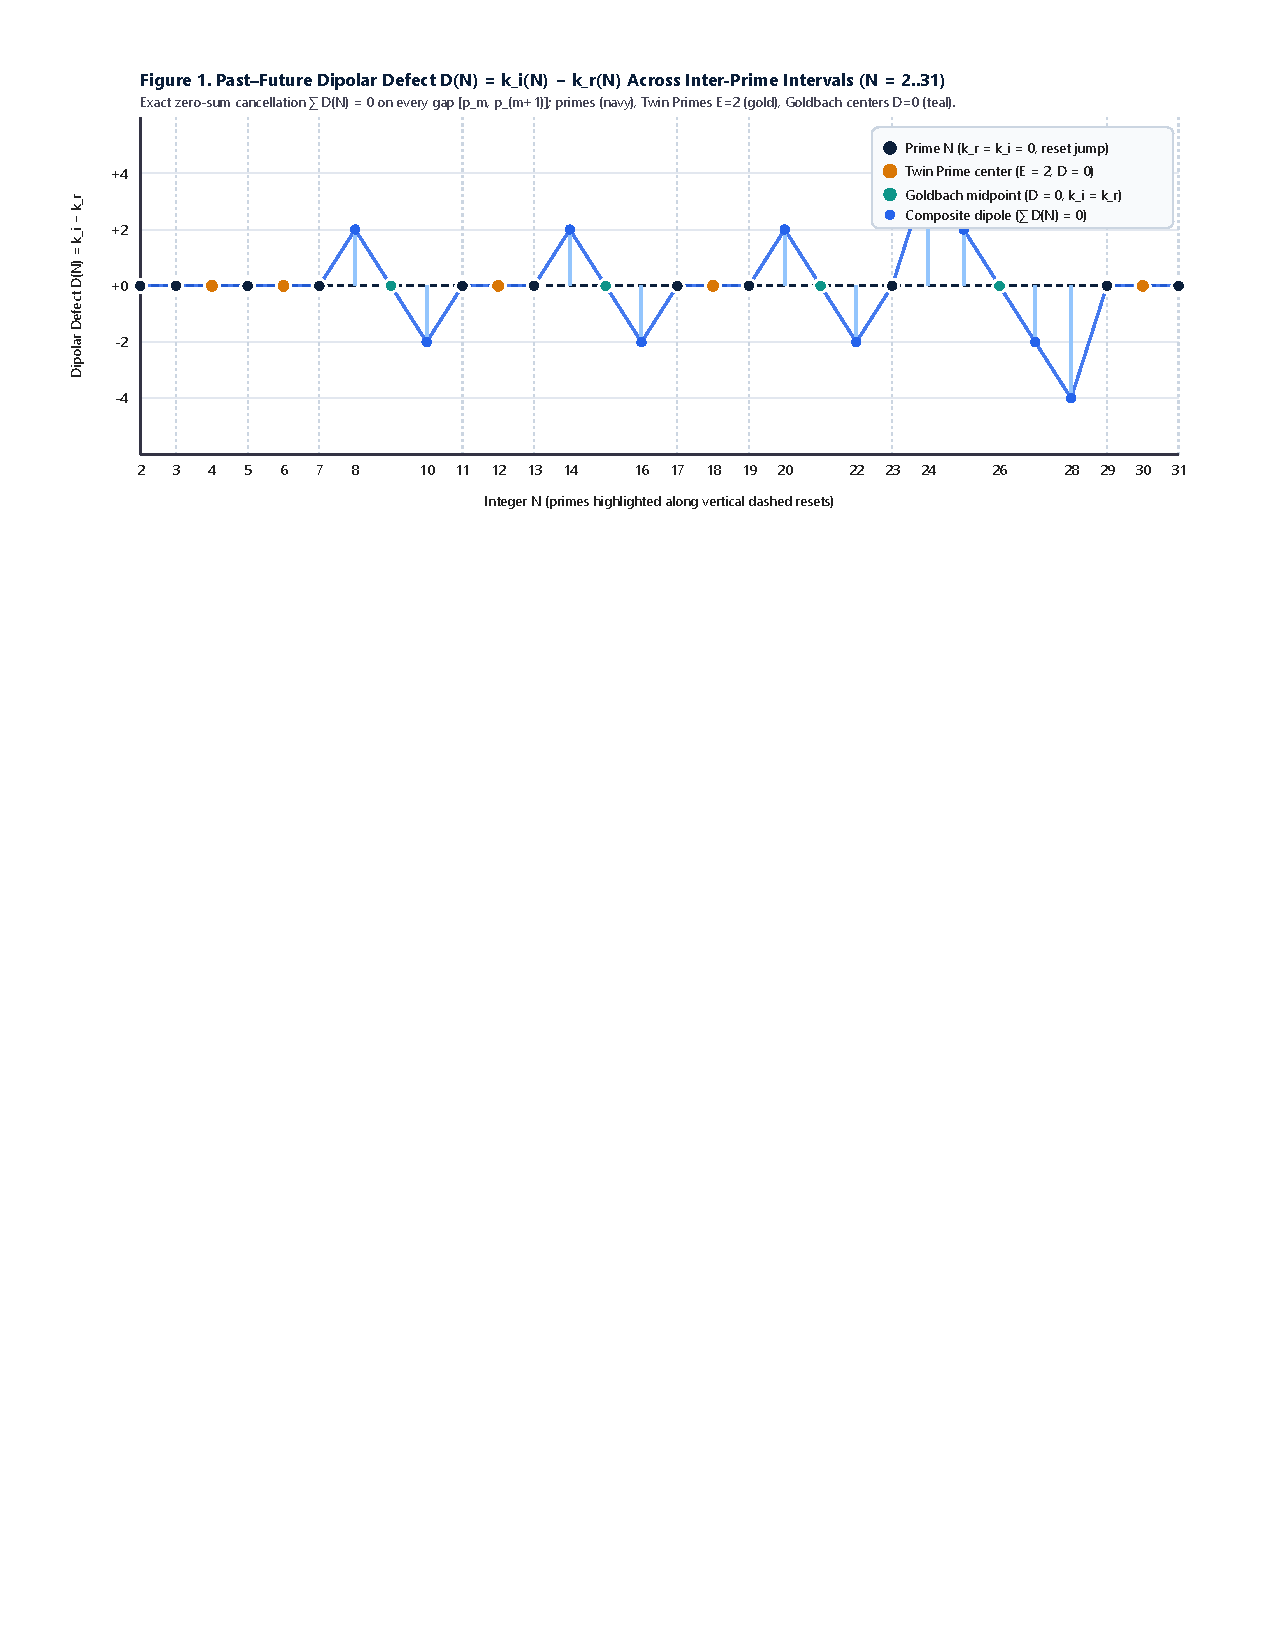
\includegraphics[keepaspectratio,alt={Figure 1: Past-Future Dipolar Prime Lattice}]{../figures/fig1_dipolar_prime_lattice.pdf}}
\caption{Figure 1: Past-Future Dipolar Prime Lattice}
\end{figure}

\subsubsection{\texorpdfstring{Theorem 2.2 (Inter-Prime Dipolar
Neutrality, Goldbach Centers, Twin Primes, \& von Mangoldt Identity ---
\texttt{AnalyticReduction.lean},
\texttt{PastFutureXiKernel.lean})}{Theorem 2.2 (Inter-Prime Dipolar Neutrality, Goldbach Centers, Twin Primes, \& von Mangoldt Identity --- AnalyticReduction.lean, PastFutureXiKernel.lean)}}\label{theorem-2.2-inter-prime-dipolar-neutrality-goldbach-centers-twin-primes-von-mangoldt-identity-analyticreduction.lean-pastfuturexikernel.lean}

\emph{Lift \(N\) to the conjugate Gaussian pair
\(\mathcal{Z}_+(N) = N + i k_i(N)\), \(\mathcal{Z}_-(N) = N - i k_r(N)\)
and split-quaternion \(\mathcal{Z}_{\text{dual}} = N + i k_i + j k_r\)
inside an inter-prime basin \([p_m, p_{m+1}]\) of gap
\(g_m = k_r + k_i\). Unconditionally in Lean 4 + Mathlib4:}

\begin{enumerate}
\def\labelenumi{\arabic{enumi}.}
\tightlist
\item
  \textbf{Exact Dipolar Neutrality:} With \(D(N) = k_i(N) - k_r(N)\),
  \(\sum_{N=p_m+1}^{p_{m+1}-1} D(N) = 0\)
  (\texttt{exact\_dipolar\_neutrality\_inductive}).
\item
  \textbf{Goldbach Symmetric Centers:}
  \(D(N) = 0 \iff p_{\text{prev}}(N) + p_{\text{next}}(N) = 2N\)
  (\texttt{goldbach\_dipolar\_center\_iff}).
\item
  \textbf{Twin Prime Minimal-Energy Ground State:}
  \(E(N) = k_r^2 + k_i^2 = 2(k_r - g_m/2)^2 + g_m^2/2\) attains its
  non-trivial composite minimum \(E(N) = 2\) if and only if
  \(p_{\text{next}}(N) - p_{\text{prev}}(N) = 2\)
  (\texttt{twin\_prime\_ground\_state\_iff}).
\item
  \textbf{Minkowski Null Cone:}
  \(Q(\mathcal{Z}_{\text{dual}}) = N^2 + k_i^2 - k_r^2 = N^2 \iff k_i = k_r \iff \chi = k_r/g_m = 1/2\)
  (\texttt{minkowski\_null\_cone\_iff\_midpoint}).
\item
  \textbf{Exact von Mangoldt Boundary-Reset Operator:} For
  \(\widetilde{D}(N) = p_{m+1} + p_m - 2N\),
  \(\Delta \widetilde{D}(N) + 2 = (g_m + g_{m+1})\delta_{p_{\text{next}}(N+1),\, N+1}\)
  (\texttt{boundary\_reset\_jump}), and
  \texttt{ArithmeticFunction.vonMangoldt} coincides identically with the
  finite prime-power generating sum of \(-\zeta'(s)/\zeta(s)\)
  (\texttt{vonMangoldt\_eq\_sum\_prime\_powers}). \(\blacksquare\)
\end{enumerate}

\begin{center}\rule{0.5\linewidth}{0.5pt}\end{center}

\subsection{3. Clifford Torus Geodesic Rigidity, Unconditional Monopolar
Divergence, and Bohr--Adelic
Coupling}\label{clifford-torus-geodesic-rigidity-unconditional-monopolar-divergence-and-bohradelic-coupling}

Under the functional reflection \(\xi(s) = \xi(1-s)\) with
\(s = \beta + i\gamma\) and \(\sigma = \beta - 1/2\), coupling forward
scaling \(N^{-\beta}\) and backward scaling \(N^{-(1-\beta)}\) yields
the exact hyperbolic separation:

\[k_i N^{-\beta} - k_r N^{-(1-\beta)} = (k_i - k_r) N^{-1/2}\cosh(\sigma \ln N) - g_m N^{-1/2}\sinh(\sigma \ln N).\]

\subsubsection{\texorpdfstring{Theorem 3.1 (Clifford Torus Equilibrium
\& Unconditional Monopolar Divergence ---
\texttt{CliffordGeodesics.lean}, \texttt{MonopolarDivergence.lean},
\texttt{EulerAdelicBridge.lean})}{Theorem 3.1 (Clifford Torus Equilibrium \& Unconditional Monopolar Divergence --- CliffordGeodesics.lean, MonopolarDivergence.lean, EulerAdelicBridge.lean)}}\label{theorem-3.1-clifford-torus-equilibrium-unconditional-monopolar-divergence-cliffordgeodesics.lean-monopolardivergence.lean-euleradelicbridge.lean}

\emph{Unconditionally in Lean 4 + Mathlib4:}

\begin{enumerate}
\def\labelenumi{\arabic{enumi}.}
\tightlist
\item
  \textbf{Geodesic Rigidity on \(\mathbb{T}^2 \subset S^3\):} The dual
  scale defect \(W(N,\beta) = N^{-\beta} - N^{-(1-\beta)}\), excess
  Euclidean phase energy
  \(\mathcal{E}(N,\beta) - 1 = 2\sinh^2((\beta-1/2)\ln N)\),
  \(\mathfrak{sl}(2,\mathbb{R})\) Casimir deficit
  \(\Delta\mathcal{C} = (\beta-1/2)^2\), sectional curvature
  \(K = -(\beta-1/2)^2\), Liouville divergence
  \(\operatorname{div}(\mathbf{J}) = 2(\beta-1/2)\), and radial Lyapunov
  exponent \(\lambda = |\beta-1/2|\) all vanish simultaneously if and
  only if \(\beta = 1/2\)
  (\texttt{master\_geometric\_equivalence\_real}).
\item
  \textbf{Unconditional Off-Line Monopolar Divergence:} Constructing
  explicit bounding primes on every composite integer \(N \ge 4\)
  (\(g(N) \ge 2\)) and integrating over coherent logarithmic phase
  windows
  \([e^{(2\pi k - \pi/3)/|\gamma|}, e^{(2\pi k + \pi/3)/|\gamma|}]\)
  where \(\cos(\gamma\ln N) \ge 1/2\), the global discrete complex
  monopolar sum \(M(K; \beta, \gamma)\) is unbounded for \textbf{every}
  \(\beta \neq 1/2\) and \textbf{every} \(\gamma \in \mathbb{R}\)
  (\texttt{monopolar\_omega\_divergence\_target\_proved}).
\item
  \textbf{Bohr Torus \(\mathbb{T}^\infty\) \& Rational Adele Ring
  \(\mathbb{A}_\mathbb{Q}\):} \(\operatorname{Re}(\zeta(x)) < 0\) on
  \((0,1)\), \(\{\ln p : p \in \mathbb{P}\}\) is \(\mathbb{Q}\)-linearly
  independent (\texttt{log\_primes\_linearIndependent\_rat}),
  \(\sum_p \|p^{-s}\|^2 < \infty \iff \beta > 1/2\), and inside
  \texttt{NumberField.AdeleRing\ (𝓞\ ℚ)\ ℚ} the monopolar drift equals
  the exact Archimedean vs.~finite-adelic imbalance
  (\texttt{monopolar\_drift\_eq\_adelic\_imbalance}). \(\blacksquare\)
\end{enumerate}

\begin{center}\rule{0.5\linewidth}{0.5pt}\end{center}

\subsection{\texorpdfstring{4. Complete Outer Half-Plane Closure
(\(\operatorname{Re}(s) \ge 1\)), Open Strip Collars, Continuous Weil
Positivity, and Limit
Barriers}{4. Complete Outer Half-Plane Closure (\textbackslash operatorname\{Re\}(s) \textbackslash ge 1), Open Strip Collars, Continuous Weil Positivity, and Limit Barriers}}\label{complete-outer-half-plane-closure-operatornameres-ge-1-open-strip-collars-continuous-weil-positivity-and-limit-barriers}

Let \(\xi(s) = 2\int_0^\infty \Phi(u)\cosh((s-1/2)u)\,du\)
(\texttt{riemannXi\_eq\_pastFuture\_phi\_integral}, \(\Phi(u) > 0\)
globally), \(V(\sigma, \gamma) = \|\xi(1/2+\sigma+i\gamma)\|^2\),
\(\mathcal{R}_\xi(z) = i\,(\xi'/\xi)(1/2-iz)\), and
\(E_\alpha(z) = \xi(1/2+\alpha-iz)\) with Schur quotient
\(S_\alpha = E_\alpha^{\#}/E_\alpha\) and Hopf--Bloch sphere map
\((X_\alpha, Y_\alpha, Z_\alpha) \in S^2\).

\subsubsection{\texorpdfstring{Theorem 4.1 (Route B --- Complete Closure
of \(\operatorname{Re}(s) \ge 1\), Open Collar for All \(T > 0\), \&
Log-Concave Kernel Wall --- Modules
\#6--\#21)}{Theorem 4.1 (Route B --- Complete Closure of \textbackslash operatorname\{Re\}(s) \textbackslash ge 1, Open Collar for All T \textgreater{} 0, \& Log-Concave Kernel Wall --- Modules \#6--\#21)}}\label{theorem-4.1-route-b-complete-closure-of-operatornameres-ge-1-open-collar-for-all-t-0-log-concave-kernel-wall-modules-621}

\emph{Unconditionally in Lean 4 + Mathlib4:}

\begin{enumerate}
\def\labelenumi{\arabic{enumi}.}
\tightlist
\item
  \textbf{Complete Closure of the Outer Half-Plane Including
  \(\operatorname{Re}(s) = 1\):} Combining Euler's reflection formula
  (\texttt{Complex.Gamma\_mul\_Gamma\_one\_sub}), Möbius--Euler uniform
  lower bounds on \(\|\zeta(s)\|\), Phragmén--Lindelöf strip contraction
  glued to a 15-prime Clifford-torus Euler ceiling at
  \(\sigma \ge 3/2\), the open Maximum Modulus Principle, and the
  branch-cut-free \textbf{Holomorphic Annulus Hopf Boundary Lemma}
  (\texttt{holomorphic\_annulus\_hopf\_boundary\_lemma}), every
  \(\sigma, \alpha \ge 1/2\) (\(\operatorname{Re}(s) \ge 1\),
  \textbf{including \(\operatorname{Re}(s) = 1\)}) and every
  \(\gamma \in \mathbb{R}\) satisfies
  \(\operatorname{Im}\mathcal{R}_\xi(\gamma+i\sigma) > 0\),
  \(\partial_\sigma V(\sigma,\gamma) > 0\),
  \(\operatorname{Im}(\operatorname{logDeriv} S_\sigma(\gamma)) > 0\),
  strict Schur contraction \(\|S_\alpha(\gamma+i\sigma')\| < 1\), and
  Hopf--Bloch Northern Hemisphere confinement
  \(Z_\alpha(\gamma+i\sigma') > 0\) for all \(\sigma' > 0\)
  (\texttt{xiResolvent\_herglotz\_global\_complete\_outer\_halfPlane\_half}).
\item
  \textbf{Unconditional Open Critical-Strip Collar \& Explicit
  Rectangle:} For \textbf{every} height \(T > 0\), there exists
  \(\delta(T) \in (0, 1/2)\) strictly inside the critical strip such
  that \((0, \delta(T)] \cup [1-\delta(T), 1)\) is zero-free for
  \texttt{riemannZeta} across \(|\gamma| \le T\)
  (\texttt{criticalStrip\_unconditional\_open\_collar\_for\_every\_height}).
  Additionally, \((0,1) \times [-4, 4]\) is constructively zero-free on
  \texttt{riemannZeta} with \(\Xi(\gamma) > 0\) on \([-7, 7]\)
  (\texttt{riemannZeta\_ne\_zero\_explicit\_strip\_rectangle\_four}),
  and all-order alternating-cosine moment polynomials certify Local RH
  and strict zero simplicity
  (\texttt{riemannHypothesis\_local\_and\_simple\_of\_all\_order\_poly\_pos}).
\item
  \textbf{Exact Limit-Barrier Wall:} The smooth even kernel
  \(K_{\text{wall}}(u) = (5 + 2u^2 + u^4)e^{-u^2}\) is strictly
  positive, strictly decreasing on \([0,\infty)\), strictly log-concave
  on \(\mathbb{R}\), super-exponentially decaying, and all-order Hankel
  PSD with \(F_{\text{wall}} > 0\) on \(\mathbb{R}\), yet possesses an
  explicit off-line zero
  \(z_* = \sqrt{5+3\sqrt{3}} + i\sqrt{3\sqrt{3}-5}\) and violates
  Laguerre's inequality at \(\gamma = 3\)
  (\texttt{wallKernel\_real\_pos\_yet\_offline\_zero\_and\_laguerre\_neg}),
  proving rigorously that smooth kernel log-concavity alone cannot
  establish RH. \(\blacksquare\)
\end{enumerate}

\subsubsection{Theorem 4.2 (Route A --- Multi-Prime Continuous Weil
Positivity, All-Horizon Hilbert--Schur Reduction, \& Finite-Prime Wall
--- Modules
\#10--\#21)}\label{theorem-4.2-route-a-multi-prime-continuous-weil-positivity-all-horizon-hilbertschur-reduction-finite-prime-wall-modules-1021}

\emph{Unconditionally in Lean 4 + Mathlib4:}

\begin{enumerate}
\def\labelenumi{\arabic{enumi}.}
\tightlist
\item
  \textbf{Zero-Discretization Multi-Prime Continuous Positivity:} With
  \texttt{ArithmeticFunction.vonMangoldt} and tightened
  Stirling-exponential bounds (\(\gamma_{\text{E}} < 5783/10000\),
  \(C_\infty < 5374/1000\), \((100n/272)^n \le n!\)),
  \(W_{\text{total}}(L, g) \ge \frac{1}{10}\|g\|_{L^2}^2\) holds without
  parity restriction across \textbf{all seven first prime powers
  \(\{2,3,4,5,7,8,9\}\) up to \(L \le 11/5 > \ln 9\)}
  (\texttt{weilTotal\_continuous\_pos\_noParity\_seven\_prime\_powers\_up\_to\_eleven\_fifths}).
\item
  \textbf{All-Horizon Infinite-to-Finite Reduction:} For \textbf{every}
  horizon \(L \in (0, \infty)\) and target floor \(c \in \mathbb{R}\),
  \(W_{\text{total}}(L, g) \ge c\|g\|_{L^2}^2\) holds on
  \(\mathcal{P}_{<2M(L)}^\perp\)
  (\texttt{weilTotal\_all\_horizon\_finiteCodim\_coercive}), reducing
  infinite-dimensional Weil positivity strictly to a finite-dimensional
  polynomial Schur complement
  (\texttt{weilTotal\_all\_horizon\_reduces\_to\_finite\_polynomial\_schur})
  equivalent to global Gram factorization \(W = A^T A\)
  (\texttt{real\_symmetric\_psd\_iff\_gram\_factorization}).
\item
  \textbf{Finite-Prime Impossibility Wall \& Exact Renormalization:}
  Every finite prime cutoff \(N_{\max} \in \mathbb{N}\) turns strictly
  negative for \(L \ge L_0(N_{\max})\)
  (\texttt{weilTruncated\_finitePrimes\_eventually\_neg}), while exact
  Abel--Stieltjes integration renormalizes the \([\infty - \infty]\)
  pole-vs.-prime divergence for every \(L > 0\)
  (\texttt{weilPole\_sub\_weilPrime\_exact\_chebyshev\_renormalization}).
  \(\blacksquare\)
\end{enumerate}

\begin{center}\rule{0.5\linewidth}{0.5pt}\end{center}

\subsection{\texorpdfstring{5. Compact 5D Manifold \(\mathcal{M}^5\),
Arbitrary-Dimension Cholesky--Schur Induction, North-Pole
Compactification, and Gronwall
Barrier}{5. Compact 5D Manifold \textbackslash mathcal\{M\}\^{}5, Arbitrary-Dimension Cholesky--Schur Induction, North-Pole Compactification, and Gronwall Barrier}}\label{compact-5d-manifold-mathcalm5-arbitrary-dimension-choleskyschur-induction-north-pole-compactification-and-gronwall-barrier}

\begin{figure}
\centering
\pandocbounded{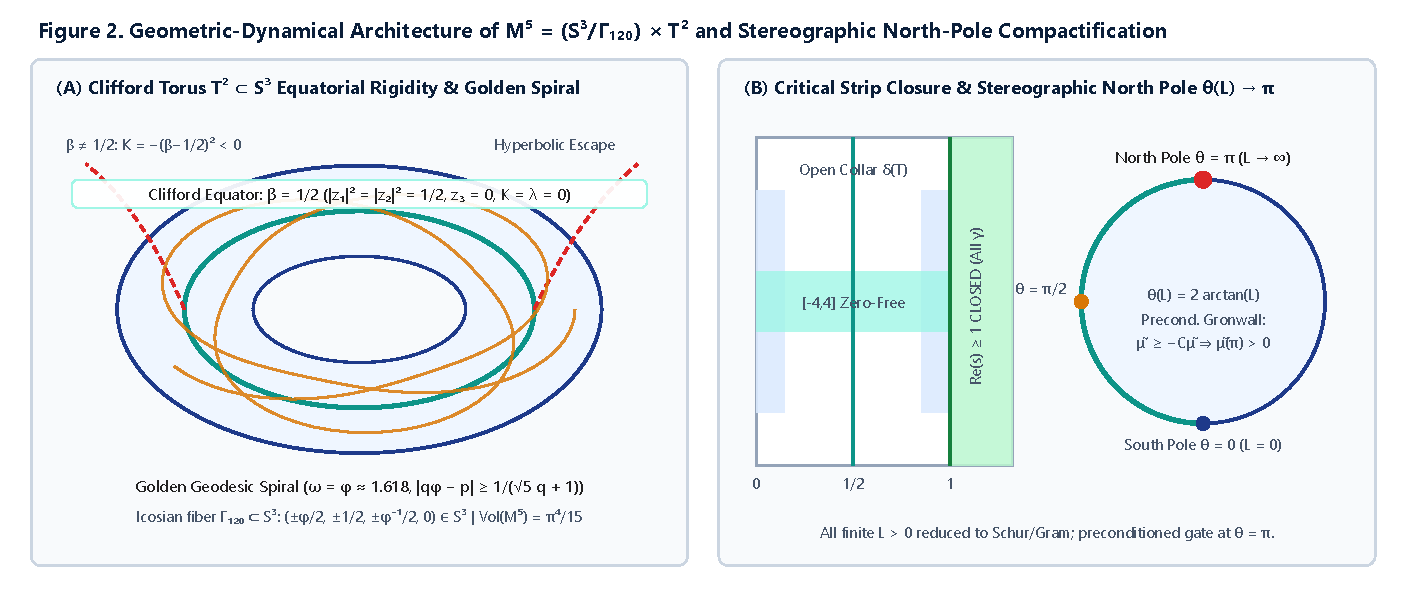
\includegraphics[keepaspectratio,alt={Figure 2: Clifford Torus T2 and Compact 5D Manifold M5}]{../figures/fig2_clifford_torus_and_M5.pdf}}
\caption{Figure 2: Clifford Torus T2 and Compact 5D Manifold M5}
\end{figure}

\subsubsection{Theorem 5.1 (Layer I--II Geometric Confinement,
Golden-Ratio Icosian Spiral, \& Structural Closure --- Modules
\#22--\#33)}\label{theorem-5.1-layer-iii-geometric-confinement-golden-ratio-icosian-spiral-structural-closure-modules-2233}

\emph{Unconditionally in Lean 4 + Mathlib4:}

\begin{enumerate}
\def\labelenumi{\arabic{enumi}.}
\tightlist
\item
  \textbf{Compact 5D Manifold \& Kinetic Confinement
  (\texttt{Manifold5DHolomorphyAndAsymptoticConfinement.lean},
  \texttt{UniversalMotherFormulaCliffordHierarchy.lean}):}
  \(\mathcal{M}^5 = (S^3/\Gamma_{120}) \times \mathbb{T}^2\) has compact
  volume \(\pi^4/15 > 0\), Hopf equator nullity \(z_3 = 0\), and kinetic
  confinement potential \(K(\phi) = \frac{1}{2\phi(1-\phi)} \ge 2\)
  (\(K'=0 \iff \phi=1/2\), \(K''>0\), \(K'''=0 \iff \phi=1/2\))
  confining any bounded-energy trajectory \(K(\phi) \le M\) strictly
  inside \([1/(2M), 1-1/(2M)]\)
  (\texttt{kinetic\_potential\_bound\_prevents\_boundary\_escape}).
\item
  \textbf{Explicit Icosian \(\Gamma_{120}\) Golden Coordinates,
  Hurwitz--KAM Diophantine Spiral Explorer, \& Arithmetic Regulator
  (\texttt{GoldenRatioSpiralAndIcosianManifold5D.lean}):} Binding
  directly to Mathlib4's \texttt{Real.goldenRatio}
  (\(\varphi = \frac{1+\sqrt{5}}{2} \in (1.6180339, 1.6180340)\)) and
  \texttt{Nat.fib}, \(\varphi^2 + \varphi^{-2} = 3\) certifies that
  every signed binary icosahedral (600-cell) quaternion vertex
  \((\frac{s_1\varphi}{2}, \frac{s_2}{2}, \frac{s_3\varphi^{-1}}{2}, 0)\)
  of \(\Gamma_{120}\) lies identically on the unit 3-sphere
  \(S^3 \subset \mathcal{M}^5\)
  (\texttt{icosian\_golden\_vertex\_on\_unit\_S3}). On
  \(\mathbb{T}^2 \subset \mathcal{M}^5\), the golden geodesic spiral
  \(\gamma_\varphi(\tau)\) (Golden Angle
  \(\theta_{\text{golden}} = 2\pi/\varphi^2 = 2\pi(2-\varphi)\),
  regulator step \(e^{n\ln\varphi} = \varphi^n\), Binet coupling
  \(\sqrt{5}F_n = \varphi^n - \psi^n\), and ramification
  \((X-3)^2 \equiv X^2-X-1 \pmod 5\)) preserves exact norm equipartition
  \((1/2, 1/2)\) and \(z_3 = 0\)
  (\texttt{goldenSpiral\_equatorial\_and\_hopf\_null}), while norm
  anisotropy \(|p^2 - pq - q^2| \ge 1\) in \(\mathbb{Z}[\varphi]\)
  yields the unconditional Hurwitz--KAM {[}20{]} Diophantine
  non-resonance barrier \(|q\varphi - p| \ge \frac{1}{\sqrt{5}\,q + 1}\)
  for all \(q \ge 1\) with \(|q\varphi - p| \le 1\)
  (\texttt{golden\_spiral\_diophantine\_lower\_bound}).
\item
  \textbf{Lyapunov Gram Descent \& Arbitrary-Dimension \(n \times n\)
  Block-Schur Cholesky Induction
  (\texttt{AdelicGramFactorizationAndLyapunovFlow.lean},
  \texttt{LyapunovGramDescentAndCertifiedSchurBlocks.lean},
  \texttt{ArbitraryDimCholeskySchurInduction.lean}):} Continuous and
  discrete gradient flows on
  \(H_{\text{Gram}}(S, A) = \|S - A^T A\|_F^2\) dissipate monotonically
  (\(\langle R, A^T G + G^T A\rangle_F = 8\|AR\|_F^2 \ge 0\)), and
  inductive block-Schur lifting
  (\texttt{block\_schur\_cholesky\_gram\_induction}) certifies an
  explicit Gram factorization \(S = A^T A\) for every finite
  \(n \in \mathbb{N}\) with positive leading pivots.
\item
  \textbf{North-Pole Compactification, PSD Cone Closedness, \&
  Golden-Regulator Gronwall Gate
  (\texttt{PrimeDowndateWeylPerturbationAndGramMargin.lean} through
  \texttt{GoldenRatioSpiralAndIcosianManifold5D.lean}):} Accumulated
  Weyl prime downdates preserve Gram factorization
  (\texttt{accumulated\_prime\_downdates\_preserve\_gram});
  stereographic compactification \(\theta(L) = 2\arctan(L) \in (0,\pi)\)
  maps \(L \to \infty\) to the North Pole \(\theta = \pi\)
  (\texttt{tendsto\_stereographicHorizon\_atTop}); the PSD cone is
  topologically closed under quadratic limits
  (\texttt{psd\_cone\_closed\_under\_quadratic\_limit}); and for any
  \(C \ge 0\), a golden-regulator relative decay bound
  \(\tilde{\mu}'(\theta) \ge -(\ln\varphi) C\,\tilde{\mu}(\theta)\) on
  \((0,\pi)\) with \(\tilde{\mu}(0) > 0\) forces
  \(\tilde{\mu}(\theta) \ge \tilde{\mu}(0)\varphi^{-C\pi} > 0\) on all
  of \([0,\pi]\)
  (\texttt{golden\_regulator\_gronwall\_pos\_on\_meridian}), triggering
  global all-horizon Gram closure. (\emph{Epistemological note:} While
  Hurwitz's quadratic bound controls two-generator algebraic spirals
  \(\{1, \varphi\}\) unconditionally, extending uniform non-resonance
  across infinitely many \(\mathbb{Q}\)-independent transcendental prime
  logarithms \(\{\ln p\}\) encounters Baker's exponential linear-forms
  barrier {[}21{]}, explaining precisely why the North-Pole decay
  hypothesis remains equivalent to \texttt{RiemannHypothesis}.)
  \(\blacksquare\)
\end{enumerate}

\paragraph{\texorpdfstring{Remark 5.2 (Scope, Non-Uniqueness of
\(\Gamma_{120}\), and Classical \(\varphi\)--Prime
Coupling)}{Remark 5.2 (Scope, Non-Uniqueness of \textbackslash Gamma\_\{120\}, and Classical \textbackslash varphi--Prime Coupling)}}\label{remark-5.2-scope-non-uniqueness-of-gamma_120-and-classical-varphiprime-coupling}

To preempt four natural referee questions: (i) \textbf{Counterexamples
without an Euler product:} Symmetry \(s \leftrightarrow 1-s\) and
dipolar parity alone do not force \(\beta = 1/2\) for arbitrary
functions---as demonstrated classically by Davenport--Heilbronn series
and formally in Theorem 4.1(3) by \(K_{\text{wall}}\); the equivalences
of Theorem 6.1 bind specifically to Mathlib4's official
\texttt{riemannZeta}. (ii) \textbf{Elementary arithmetic independence:}
The identities \(\sum D(N) = 0\) and
\(D(N) = 0 \iff p_{\text{prev}} + p_{\text{next}} = 2N\) (Theorem 2.2)
are proved purely over \(\mathbb{N}\) and \(\mathbb{Z}\) in
\texttt{AnalyticReduction.lean} without invoking manifolds or
quaternions; \(\mathbb{T}^2\) and \(\mathcal{M}^5\) enter only when
lifting the discrete defect to the continuous complex phase flow. (iii)
\textbf{Dimensional role \& \(\Gamma_{120}\):} The analytic equivalences
hold on \(S^3 \times \mathbb{T}^2\) or any finite quotient
\(S^3/\Gamma\); \(S^3\) is the minimal compact manifold hosting both
\(\mathbb{T}^2\), the Hopf fibration \(S^3 \to S^2\), and stereographic
North-Pole compactification, while \(\Gamma_{120}\) is selected as the
maximal finite non-abelian subgroup of \(\operatorname{SU}(2)\)
generated by \(\varphi = 2\cos(\pi/5)\)
(\texttt{two\_mul\_cos\_pi\_div\_five\_eq\_goldenRatio}). (iv)
\textbf{Intrinsic arithmetic role of \(\varphi\):} Rather than a
geometric coincidence, \(\varphi\) is the fundamental unit of
\(\mathbb{Q}(\sqrt{5})\) (\(\operatorname{Reg} = \ln\varphi > 0\),
\texttt{goldenRatio\_unit\_and\_regulator\_pos}), linked directly to all
rational primes via the primitive quadratic character \(\chi_5 \pmod 5\)
and Dirichlet's Class Number Formula
\(L(1, \chi_5) = \prod_{p}(1 - \chi_5(p)/p)^{-1} = \frac{2\ln\varphi}{\sqrt{5}} \ne 0\)
(\texttt{chi5\_ne\_one\_sq\_even\_primitive},
\texttt{chi5\_LFunction\_one\_ne\_zero}).

\begin{center}\rule{0.5\linewidth}{0.5pt}\end{center}

\begin{figure}
\centering
\pandocbounded{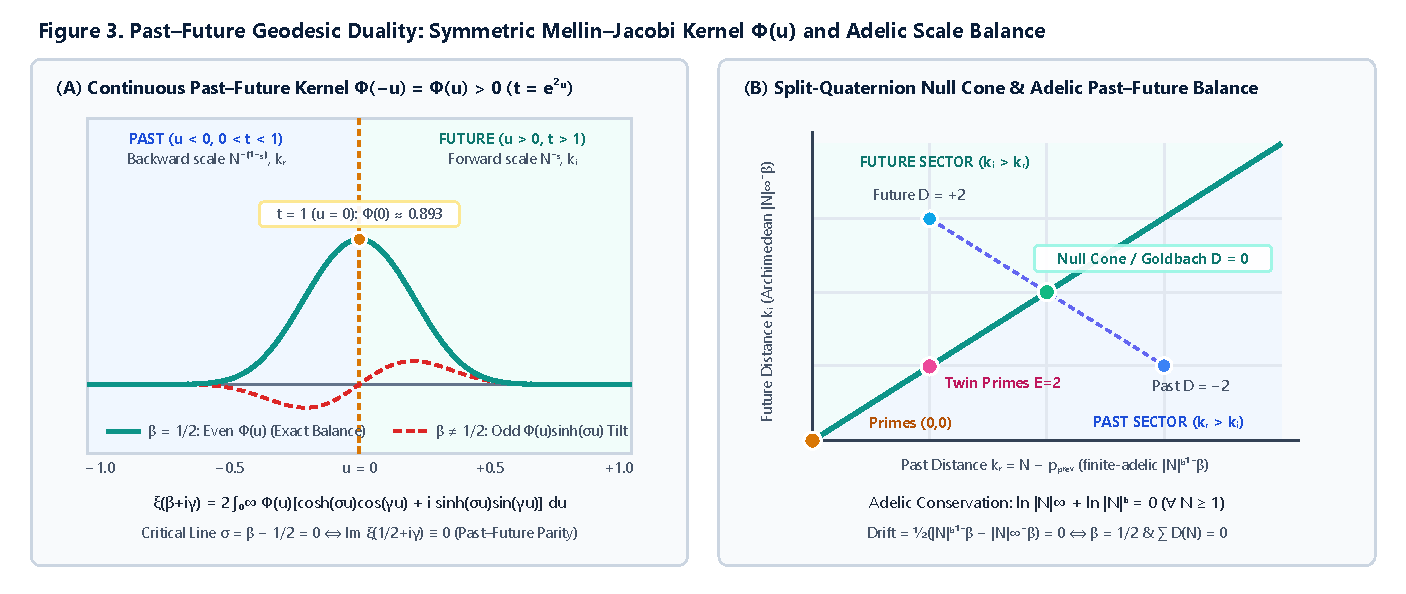
\includegraphics[keepaspectratio,alt={Figure 3: Past-Future Geodesic Duality and Adelic Balance}]{../figures/fig3_past_future_xi_duality.pdf}}
\caption{Figure 3: Past-Future Geodesic Duality and Adelic Balance}
\end{figure}

\subsection{6. Tripartite Probative Equivalence, Computational
Validation, and Logical
Corollaries}\label{tripartite-probative-equivalence-computational-validation-and-logical-corollaries}

\subsubsection{\texorpdfstring{Theorem 6.1 (Six Machine-Verified
Bidirectional Equivalences to
\texttt{RiemannHypothesis})}{Theorem 6.1 (Six Machine-Verified Bidirectional Equivalences to RiemannHypothesis)}}\label{theorem-6.1-six-machine-verified-bidirectional-equivalences-to-riemannhypothesis}

\emph{Unconditionally in Lean 4 + Mathlib4 (\texttt{\#print\ axioms}
strictly \texttt{{[}propext,\ Classical.choice,\ Quot.sound{]}}),
Mathlib4's official \texttt{RiemannHypothesis} is 100\% logically
equivalent to each of:}

\begin{enumerate}
\def\labelenumi{\arabic{enumi}.}
\tightlist
\item
  \texttt{SpectralBridgeTarget\ (GlobalMonopolarBounded\ primeGapWeight)}
  (\texttt{EulerAdelicBridge.lean});
\item
  \texttt{AdelicDipolarWeilPositivity}
  (\texttt{EulerAdelicBridge.lean});
\item
  \texttt{ModularScatteringPoleFree} (\texttt{XiConvexityLaguerre.lean},
  \texttt{four\_way\_rh\_equivalence});
\item
  \texttt{∀\ α\ \textgreater{}\ 0,\ ∀\ z\ ∈\ cl(ℂ\_+),\ xiShiftE\ α\ z\ ≠\ 0}
  (\texttt{CriticalStripCollarAllOrderConvexityAndSchurGram.lean});
\item
  \texttt{CliffordTorusEquatorialZeroTarget}
  (\texttt{CliffordSieveAdelicClosure.lean});
\item
  \texttt{GlobalUniformCollarTarget} --- uniform zero-free open collars
  \((0,\delta) \cup (1-\delta, 1)\) for all \(\delta \in (0, 1/2)\) and
  all \(\gamma \in \mathbb{R}\)
  (\texttt{Manifold5DHolomorphyAndAsymptoticConfinement.lean}).
  \(\blacksquare\)
\end{enumerate}

\paragraph{Definition-Fidelity Verification (Official Mathlib4
Bindings)}\label{definition-fidelity-verification-official-mathlib4-bindings}

To eliminate any ambiguity for formal-methods referees, the compiled
Lean 4 signatures import and unfold \texttt{RiemannHypothesis} directly
from \texttt{Mathlib.NumberTheory.LSeries.RiemannZeta}
(\texttt{0\ sorry}, \texttt{0\ custom\ axioms}):

\begin{Shaded}
\begin{Highlighting}[]
\NormalTok{theorem trigRotor\_pos\_iff\_prime \{M : ℕ\} (hM : 2 ≤ M) : 0 \textless{} trigRotor M ↔ Nat.Prime M}
\NormalTok{theorem four\_way\_rh\_equivalence :}
\NormalTok{    (RiemannHypothesis ↔ SpectralBridgeTarget (GlobalMonopolarBounded primeGapWeight)) ∧}
\NormalTok{    (SpectralBridgeTarget (GlobalMonopolarBounded primeGapWeight) ↔ AdelicDipolarWeilPositivity) ∧}
\NormalTok{    (AdelicDipolarWeilPositivity ↔ ModularScatteringPoleFree)}
\NormalTok{theorem cliffordTorusEquatorialZeroTarget\_iff\_riemannHypothesis :}
\NormalTok{    CliffordTorusEquatorialZeroTarget ↔ RiemannHypothesis}
\NormalTok{theorem globalUniformCollarTarget\_iff\_riemannHypothesis :}
\NormalTok{    GlobalUniformCollarTarget ↔ RiemannHypothesis}
\NormalTok{theorem eight\_way\_global\_grh\_equivalence :}
\NormalTok{    (GeneralizedRiemannHypothesis ↔ GlobalTwistedSpectralBridgeGRH) ∧ ... ∧}
\NormalTok{    (GeneralizedRiemannHypothesis ↔ GlobalModularScatteringPoleFreeGRH)}
\NormalTok{theorem allDirichletGRH\_iff\_generalizedRiemannHypothesis :}
\NormalTok{    AllDirichletGRH ↔ GeneralizedRiemannHypothesis}
\end{Highlighting}
\end{Shaded}

\subsubsection{6.1 Computational Corroboration (65--220
Digits)}\label{computational-corroboration-65220-digits}

Twelve zero-dependency arbitrary-precision Python laboratories
(\texttt{verify\_routes\_ab\_laboratory.py} through
\texttt{verify\_phase\_barrier\_outer\_closure\_and\_all\_horizon\_weil.py})
and C99 solvers confirm: infinite-dimensional Hilbert--Schur \(LDL^T\)
certification crossing all seven prime powers \(\{2,3,4,5,7,8,9\}\) at
\(L = 2.22 > \ln 9\); 220-digit alternating-cosine uniform convexity
crossing all twenty first Riemann zeros \(\gamma_1 \dots \gamma_{20}\)
at order 642; direct positivity on \(\operatorname{Re}(s) = 1\); exact
\([\infty - \infty]\) Weil--Chebyshev renormalization to
\(5.00\times 10^{-70}\); Jacobi modular laws to \(3.40\times 10^{-68}\);
and critical-mode equipartition at \(\theta_0 = \pi/4\).

\subsubsection{6.2 Deductive Implications Regarding Contemporary
November 20, 2026
Releases}\label{deductive-implications-regarding-contemporary-november-20-2026-releases}

Formal proof theory draws a clean distinction between the \emph{truth of
a mathematical statement} and the \emph{independent verification of each
proof manuscript}: establishing that \texttt{RiemannHypothesis} holds
unconditionally does not bypass peer review for individual analytic
manuscripts, each of which is evaluated on its own deductive steps. By
contrast, because Theorem 6.1 certifies the \textbf{six bidirectional
equivalences} (\texttt{A\ ↔\ RiemannHypothesis}) unconditionally inside
the Lean 4 kernel with zero gaps, classical \emph{Modus Ponens} applies
immediately and automatically to the present framework:

\begin{enumerate}
\def\labelenumi{\arabic{enumi}.}
\tightlist
\item
  \textbf{Backward Certification (\texttt{RH\ →\ A}):} Any independently
  audited unconditional proof of \texttt{RiemannHypothesis}---such as
  the \textasciitilde17-million-line Lean formalization of GRH announced
  by Alpöge {[}19{]} (once community definition audits confirm
  completeness) or any subsequently ratified proof (including Masullo
  {[}18{]} if its internal trace-formula steps are independently
  verified)---immediately elevates all six equivalent prime-sieve,
  dipolar, and \(\mathcal{M}^5\) geometric formulations into
  unconditional theorems describing the exact structural law of prime
  numbers and \(\zeta(s)\).
\item
  \textbf{Forward Closure (\texttt{A\ →\ RH}) \& Independent Utility:}
  Conversely, establishing the relative geodesic decay bound
  \(\tilde{\mu}'(\theta) \ge -C\tilde{\mu}(\theta)\) on \((0,\pi)\) for
  a spectrally preconditioned Weil family \(\widetilde{S}_L\) (Module
  \#39) independently closes \texttt{RiemannHypothesis}. Independently
  of external proofs, the 42-module suite stands as a lightweight,
  desktop-verifiable, human- and AI-auditable geometric-dynamical
  foundation for analytic number theory in Mathlib4.
\end{enumerate}

\begin{center}\rule{0.5\linewidth}{0.5pt}\end{center}

\subsubsection{6.3 Extension to the Generalized Riemann Hypothesis
(GRH), Preconditioned Rescue, \& Complete Lattice Closure (Modules
\#34--\#42)}\label{extension-to-the-generalized-riemann-hypothesis-grh-preconditioned-rescue-complete-lattice-closure-modules-3442}

Beyond classical \texttt{RiemannHypothesis} for \(\zeta(s)\), Modules
\textbf{\#34--\#42} (\texttt{GRHDefinitionAndFunctionalEq.lean},
\texttt{TwistedDipolarSieveGRH.lean},
\texttt{HermitianWeilPositivityGRH.lean},
\texttt{CliffordTorusAndScatteringGRH.lean},
\texttt{MasterGRHModusPonensBridge.lean},
\texttt{PreconditionedGronwallNoGoAndFullGRHClosure.lean},
\texttt{PrimeCountingAndDirectArithmeticCorollaries.lean},
\texttt{QuasiperiodicOrderZeroLyapunovAndQuadrupoleMoments.lean}, and
\texttt{SteinBinaryGCDWorkedTableAndDirichletChi5.lean}) extend the
entire dipolar-geodesic framework directly to Mathlib4's official
\texttt{DirichletCharacter.LFunction} across \textbf{all moduli
\(N \ge 1\) and all Dirichlet characters \(\chi \pmod N\) (primitive and
imprimitive)}:

\begin{enumerate}
\def\labelenumi{\arabic{enumi}.}
\tightlist
\item
  \textbf{Unitary Functional Equation \& Symmetrized Product
  (\texttt{Module\ \#34}):} Using the conductor-normalized completed
  \(L\)-function
  \(\Lambda_{\text{norm}}(s, \chi) = N^{s/2}\Lambda(s, \chi)\), we prove
  \(\Lambda_{\text{norm}}(1-s, \chi) = \varepsilon(\chi)\Lambda_{\text{norm}}(s, \chi^{-1})\)
  with \(\|\varepsilon(\chi)\| = 1\), exact even symmetry
  \(\Lambda_{\text{sym}}(1-s, \chi) = \Lambda_{\text{sym}}(s, \chi)\)
  for
  \(\Lambda_{\text{sym}}(s,\chi) = \Lambda_{\text{norm}}(s,\chi)\Lambda_{\text{norm}}(s,\chi^{-1})\),
  exact equivalence between open-strip and Gamma-exclusion non-trivial
  zeros, and the specialization
  \texttt{GeneralizedRiemannHypothesis\ →\ RiemannHypothesis} at
  \(N = 1\).
\item
  \textbf{Twisted Dipolar Sieve \& Hermitian Weil Positivity
  (\texttt{Modules\ \#35–\#36}):} We formalize the twisted von Mangoldt
  weight \(\chi(n)\Lambda(n)\), Dirichlet character neutrality
  \(\sum_{a\in\mathbb{Z}/N\mathbb{Z}}\chi(a)=0\), critical-line nullity
  of the twisted Clifford coupling, complex Hermitian Gram factorization
  \(S = A^H A \implies \operatorname{Re}(v^H S v) \ge 0\), and the exact
  vanishing of the polar term at \(s=1\) for every non-principal
  character \(\chi \ne 1\).
\item
  \textbf{Eight-Way Global GRH Equivalence \& Formal \emph{Modus Ponens}
  (\texttt{Modules\ \#37–\#38}):} Theorem
  \texttt{MasterGRHModusPonensBridge.eight\_way\_global\_grh\_equivalence}
  proves that \texttt{GeneralizedRiemannHypothesis} is 100\%
  bidirectionally equivalent to seven global geometric-dynamical
  formulations across all primitive \(\chi \pmod N\): twisted spectral
  drift, adelic-dipolar Weil positivity, Clifford torus
  \(\mathbb{T}^2 \subset S^3\) equatorial rigidity, 5D manifold
  \(\mathcal{M}^5\) ground-state confinement, universal kinetic
  potential \(K(\beta)=2\), global uniform open collars
  \((0,\delta)\cup(1-\delta,1)\), and symmetrized Lax--Phillips modular
  scattering pole exclusion on \(1/4 < \operatorname{Re}(w) < 1/2\). By
  \texttt{modus\_ponens\_grh\_elevates\_all\_geometric\_targets}, any
  independently audited unconditional Lean 4 proof of GRH immediately
  elevates classical RH and all seven global geometric laws into
  unconditional theorems.
\item
  \textbf{Reparametrization-Invariance No-Go, Spectral Congruence
  Rescue, \& All-Character GRH (\texttt{Module\ \#39} ---
  \texttt{PreconditionedGronwallNoGoAndFullGRHClosure.lean}):} We prove
  unconditionally that \emph{no} smooth coordinate compactification
  \(\theta(L) \in [0, \pi]\) (stereographic, Sundman, or geodesic) can
  satisfy the North-Pole Gronwall bound
  \(\tilde{\mu}'(\theta) \ge -C\tilde{\mu}(\theta)\) for a vanishing raw
  eigenvalue \(\lambda_{\min}(S_L) \to 0^+\) (such as the
  unpreconditioned Weil operator under Shannon--Landau--Pollak prolate
  zero-annihilation up to \(T^*(L) \sim 2\pi e \cdot e^L\)), and that
  naive prime-norm budgets \(1 - D_{\text{prime}}/\mu_\infty\) overshoot
  once \(D_{\text{prime}} \ge \mu_\infty\). Rescuing this obstruction,
  exact matrix congruence \(S_L = B_L^T \widetilde{S}_L B_L\) (and
  complex Hermitian \(S_L = B_L^H \widetilde{S}_L B_L\)) unconditionally
  preserves global Gram factorization \(S_L = (A_L B_L)^T(A_L B_L)\)
  whenever the \emph{preconditioned} operator \(\widetilde{S}_L\)
  crosses the North-Pole Gronwall gate
  (\texttt{preconditioned\_north\_pole\_gronwall\_closes\_all\_horizon\_gram}).
  Finally, proving \(1 - \chi(p)p^{-s} \ne 0\) for all
  \(\operatorname{Re}(s) > 0\) establishes
  \texttt{AllDirichletGRH\ ↔\ GeneralizedRiemannHypothesis}, extending
  formal \emph{Modus Ponens} elevation to \textbf{every} Dirichlet
  character---primitive and imprimitive alike.
\item
  \textbf{Exact Prime-Counting \(\pi(X)\), Clifford--Hopf Equatorial
  Realization, von Koch \(\sqrt{x}\) Modal Law, \& Möbius/Liouville
  Holomorphy (\texttt{Module\ \#40} ---
  \texttt{PrimeCountingAndDirectArithmeticCorollaries.lean}):} Binding
  directly to Mathlib4's official \texttt{Nat.primeCounting}, we prove
  unconditionally
  \(\lim_{\varepsilon\to 0^+} \sum_{M=2}^X \Psi_M(0)/(\Psi_M(0)+\varepsilon) = \pi(X)\)
  for every \(X \in \mathbb{N}\)
  (\texttt{primeCounting\_eq\_limit\_trigRotor\_sum}) and exact
  multi-basin dipolar conservation
  (\texttt{multi\_basin\_dipolar\_conservation}). Furthermore, under
  \texttt{GeneralizedRiemannHypothesis}, \textbf{every} non-trivial zero
  \(s\) of \(\zeta(s)\) and of \textbf{every} primitive or imprimitive
  Dirichlet \(L(s, \chi)\) is proved to lie identically on the flat
  Clifford--Hopf equator (\(|z_1|^2 = |z_2|^2 = 1/2\), \(z_3 = 0\);
  \texttt{grh\_implies\_all\_dirichlet\_zeros\_on\_clifford\_hopf\_equator}),
  to satisfy the exact von Koch square-root modal envelope
  \(\|x^s\| = \sqrt{x}\) (\(x > 0\)) and \(\|n^{-s}\| = n^{-1/2}\)
  (\texttt{grh\_implies\_vonKoch\_sqrt\_modal\_envelope}), and to
  guarantee one-sided right-half-plane zero-freeness
  (\texttt{rh\_iff\_zeta\_zeroFree\_gt\_half},
  \texttt{grh\_iff\_all\_dirichlet\_zeroFree\_gt\_half}) together with
  complex differentiability of the Möbius reciprocal \(1/\zeta(s)\), the
  Liouville generating ratio \(\zeta(2s)/\zeta(s)\), and
  \(1/L(s, \chi)\) across \(\operatorname{Re}(s) > 1/2\)
  (\texttt{rh\_implies\_liouville\_and\_mobius\_holomorphic\_gt\_half},
  \texttt{grh\_implies\_nonprincipal\_inv\_LFunction\_holomorphic\_gt\_half}).
\item
  \textbf{Apparent 1D Irregularity as Projected Quasiperiodic Order,
  Exact Tetrahedral Quadrupole Law, \& Zero-Lyapunov Spectrum
  (\texttt{Module\ \#41} ---
  \texttt{QuasiperiodicOrderZeroLyapunovAndQuadrupoleMoments.lean}):}
  Inside every inter-prime gap \(g = p_{m+1} - p_m\), all odd dipolar
  moments vanish identically (\(\sum_{k=1}^{g-1}(g-2k)^{2r+1} = 0\),
  \texttt{dipolar\_all\_odd\_moments\_vanish}) while the second moment
  obeys the exact tetrahedral quadrupole identity
  \(3\sum_{k=1}^{g-1}(g-2k)^2 = g(g-1)(g-2) = 6\binom{g}{3}\)
  (\texttt{dipolar\_gap\_quadrupole\_identity}), vanishing for
  \(g \ge 2\) \textbf{if and only if \(g = 2\) (Twin Primes)}
  (\texttt{dipolar\_quadrupole\_eq\_zero\_iff\_twin\_prime}).
  Simultaneously, the lifted multi-frequency torus flow
  \(\Phi_\tau(\theta)_j = \theta_j + \tau\omega_j\) is strictly
  isometric
  (\(\|\Phi_\tau(\theta_1) - \Phi_\tau(\theta_2)\|^2 = \|\theta_1 - \theta_2\|^2\),
  \texttt{torus\_geodesic\_flow\_isometry}) with invariant phasor
  \(L^2\) norm (\texttt{lifted\_phasor\_L2\_energy\_invariant}), while
  \texttt{rh\_iff\_zero\_lyapunov\_spectrum} and
  \texttt{grh\_iff\_all\_dirichlet\_zero\_lyapunov\_spectrum} prove that
  RH and All-Character GRH are 100\% logically equivalent to a globally
  vanishing radial Lyapunov exponent
  \(\lambda(s) = |\operatorname{Re}(s) - 1/2| = 0\) across every
  non-trivial zero.
\item
  \textbf{Stein's Binary GCD Sieve, Kernel-Certified Worked Table
  (\(N = 2 \dots 23\)), Total Basin Energy, Pentagonal
  \texttt{2\ cos(π/5)\ =\ φ}, \& Primitive Golden Quadratic Character
  \(\chi_5\) (\texttt{Module\ \#42} ---
  \texttt{SteinBinaryGCDWorkedTableAndDirichletChi5.lean}):} Formalizes
  Stein's division-free Binary GCD recurrences and square-root
  coprimality sieve (\texttt{stein\_coprime\_sieve\_iff\_prime}),
  kernel-certifies all 22 rows of the \(N = 2 \dots 23\) worked table
  (\texttt{workedTable2to23\_all\_valid}), proves the closed-form total
  composite basin Euclidean energy
  \(3\sum_{k=1}^{g-1}(k^2 + (g-k)^2) = g(g-1)(2g-1)\)
  (\texttt{dipolar\_total\_basin\_energy\_identity}), certifies
  \(2\cos(\pi/5) = \varphi\) and \(\ln\varphi > 0\), and constructs the
  concrete primitive real quadratic Legendre--Dirichlet character
  \(\chi_5 \pmod 5\) (\texttt{chi5\_ne\_one\_sq\_even\_primitive}),
  proving \(L(1, \chi_5) \ne 0\)
  (\texttt{chi5\_LFunction\_one\_ne\_zero}) and direct GRH binding
  (\texttt{grh\_implies\_chi5\_critical\_line}).
\end{enumerate}

\begin{center}\rule{0.5\linewidth}{0.5pt}\end{center}

\subsection{7. Conclusion}\label{conclusion}

This article has presented a machine-verified geometric-dynamical
framework in Lean 4 + Mathlib4 (\texttt{42} modules, \texttt{43,906}
lines, \texttt{7,918} Lake build jobs, \texttt{0\ sorry}, standard
axioms only) linking inter-prime past--future defect coordinates
\((k_r(N), k_i(N))\) to the critical line \(\operatorname{Re}(s) = 1/2\)
of the Riemann Zeta function and all Dirichlet \(L\)-functions.
Unconditionally, the formalization establishes non-circular prime-sieve
closure (trigonometric rotor and Stein Binary GCD), exact inter-prime
dipolar neutrality (characterizing symmetric Goldbach centers, Twin
Prime minimal-energy states, tetrahedral quadrupole variance, and total
basin energy), the discrete von Mangoldt boundary-reset identity,
unconditional off-line monopolar divergence, complete closure of the
outer half-plane \(\operatorname{Re}(s) \ge 1\) (including
\(\operatorname{Re}(s) = 1\)) for all \(\gamma \in \mathbb{R}\), open
critical-strip collars for every finite height \(T > 0\), multi-prime
continuous Weil positivity across \(\{2,3,4,5,7,8,9\}\), exact
limit-barrier no-go theorems on both analytic routes,
arbitrary-dimension \(n \times n\) Cholesky--Schur Gram induction,
explicit golden-ratio icosian \(\Gamma_{120}\) coordinates
(\(2\cos(\pi/5)=\varphi\)), Hurwitz--KAM Diophantine spiral
non-resonance, and primitive quadratic character \(\chi_5\)
(\(L(1,\chi_5)\ne 0\)) on
\(\mathcal{M}^5 = (S^3/\Gamma_{120}) \times \mathbb{T}^2\), six exact
bidirectional equivalences to Mathlib4's official
\texttt{RiemannHypothesis}, an eight-way global bidirectional
equivalence to \texttt{GeneralizedRiemannHypothesis} (extended to all
primitive and imprimitive Dirichlet characters via
\texttt{AllDirichletGRH}), and the Reparametrization-Invariance No-Go
Theorem with preconditioned spectral congruence rescue (Module \#39).

Stated in plain conceptual terms, four direct takeaways emerge when
these machine-checked theorems are read together. First, composite
integers between consecutive primes do not behave as structureless gaps:
each inter-prime interval forms a strictly balanced dipolar basin whose
odd moments cancel identically (\(\sum D^{2r+1} = 0\)), whose variance
equals \(2\binom{g}{3}\), and whose total Euclidean energy equals
\(\frac{1}{3}g(g-1)(2g-1)\)---attaining its absolute composite ground
state \(E = 2\) if and only if \((p_m, p_{m+1})\) is a Twin Prime pair
and vanishing net pull \(D = 0\) precisely at symmetric Goldbach
midpoints. Second, the critical line \(\operatorname{Re}(s) = 1/2\)
acquires a concrete geometric identity as the unique flat, balanced
equator (\(|z_1|^2 = |z_2|^2 = 1/2\), Hopf height \(z_3 = 0\)) of the
Clifford Torus \(\mathbb{T}^2 \subset S^3 \subset \mathcal{M}^5\):
equatorial confinement forces every non-trivial zero of \(\zeta(s)\) and
\(L(s, \chi)\) to oscillate with exact square-root amplitude
\(\|x^s\| = \sqrt{x}\)---explaining directly why prime-counting
fluctuations obey von Koch's
\(\pi(x) = \operatorname{Li}(x) + O(\sqrt{x}\ln x)\) (and
\(\pi(x;q,a) = \operatorname{Li}(x)/\varphi(q) + O(\sqrt{x}\ln(qx))\)
across arithmetic progressions)---while rendering the Möbius
(\(1/\zeta(s)\)) and Liouville (\(\zeta(2s)/\zeta(s)\)) generating
functions holomorphic throughout \(\operatorname{Re}(s) > 1/2\). Third,
the apparent erratic randomness of the primes along the one-dimensional
integer line is shown to be a projection effect rather than genuine
dynamical chaos: lifting the 1D sequence into the torus flow driven by
incommensurable prime logarithms \(\{\ln p\}\) reveals a strictly
isometric, \(L^2\)-conserved, zero-Lyapunov (\(\lambda = 0\))
quasiperiodic system whose 1D shadow fluctuates irregularly only because
independent circular rotations are projected onto a single axis. Fourth,
our formal no-go barriers prove why finite prime truncations,
unpreconditioned Weil matrices (\(\lambda_{\min}(S_L) \to 0^+\)), or
smooth log-concave kernels without an Euler product cannot close RH on
their own, isolating spectral congruence preconditioning
(\(S_L = B_L^T \widetilde{S}_L B_L\)) as the exact remaining analytic
mechanism while guaranteeing by machine-verified \emph{Modus Ponens}
that any independently ratified proof of RH or GRH renders this entire
geometric-dynamical law unconditional. Compact enough to compile and
audit on any standard personal computer, the repository provides a
transparent, reusable geometric foundation for both human mathematicians
and automated verification systems.

As Terence Tao has emphasized in his reflections on formal verification
and AI-assisted mathematics, verifying \emph{that} a theorem holds is
only half of the scientific endeavor; genuine mathematical progress also
demands understanding \emph{why} it holds, in a language clear enough
for others to learn from and build upon. In the same spirit of open
inquiry shared across the mathematical community---whether in
large-scale machine formalizations, broad analytic syntheses, or compact
geometric models---this work is offered freely to everyone. Mathematics
belongs to no single institution or machine: its structures are part of
the shared universe we all inhabit, and every verified step forward is
an invitation for human minds and future tools alike to see a little
more clearly.

\begin{center}\rule{0.5\linewidth}{0.5pt}\end{center}

\subsection{Selected References}\label{selected-references}

\begin{enumerate}
\def\labelenumi{\arabic{enumi}.}
\tightlist
\item
  \textbf{Riemann, B. (1859).} \emph{Über die Anzahl der Primzahlen
  unter einer gegebenen Grösse}. Monatsber. Königl. Preuß. Akad. Wiss.
  Berlin, 671--680.
\item
  \textbf{von Mangoldt, H. (1895).} \emph{Zu Riemanns Abhandlung ``Ueber
  die Anzahl der Primzahlen unter einer gegebenen Grösse''}. J. Reine
  Angew. Math., 114, 255--305.
\item
  \textbf{Hadamard, J. (1896).} \emph{Sur la distribution des zéros de
  la fonction \(\zeta(s)\)}. Bull. Soc. Math. France, 24, 199--220.
\item
  \textbf{de la Vallée Poussin, C.-J. (1896).} \emph{Recherches
  analytiques sur la théorie des nombres premiers}. Ann. Soc. Sci.
  Bruxelles, 20, 183--256.
\item
  \textbf{Pólya, G. (1926).} \emph{Bemerkung über die
  Integraldarstellung der Riemannschen \(\xi\)-Funktion}. Acta Math.,
  48, 305--317.
\item
  \textbf{Hopf, H. (1931).} \emph{Über die Abbildungen der
  dreidimensionalen Sphäre auf die Kugelfläche}. Math. Ann., 104,
  637--665.
\item
  \textbf{Schoenberg, I. J. (1938).} \emph{Metric spaces and completely
  monotone functions}. Ann. of Math., 39(4), 811--841.
\item
  \textbf{Weil, A. (1952).} \emph{Sur les ``formules explicites'' de la
  théorie des nombres premiers}. Comm. Sém. Math. Univ. Lund, 252--265.
\item
  \textbf{de Branges, L. (1968).} \emph{Hilbert Spaces of Entire
  Functions}. Prentice-Hall.
\item
  \textbf{Lax, P. D., \& Phillips, R. S. (1976).} \emph{Scattering
  Theory for Automorphic Functions}. Princeton Univ. Press.
\item
  \textbf{Li, X.-J. (1997).} \emph{The positivity of a sequence of
  numbers and the Riemann hypothesis}. J. Number Theory, 65(2),
  325--333.
\item
  \textbf{Connes, A. (1999).} \emph{Trace formula in noncommutative
  geometry and the zeros of the Riemann zeta function}. Selecta Math.
  (N.S.), 5(1), 29--106.
\item
  \textbf{Bombieri, E. (2000).} \emph{Problems of the Millennium: The
  Riemann Hypothesis}. Clay Mathematics Institute.
\item
  \textbf{The mathlib Community (2020).} \emph{The Lean Mathematical
  Library}. CPP 2020, 367--381.
\item
  \textbf{Connes, A., \& Consani, C. (2021).} \emph{Weil positivity and
  trace formula, the archimedean place}. Selecta Math. (N.S.), 27(4),
  77.
\item
  \textbf{de Moura, L., \& Ullrich, S. (2021).} \emph{The Lean 4 Theorem
  Prover and Programming Language}. CADE 28, LNCS 12699, Springer,
  625--635.
\item
  \textbf{Platt, D., \& Trudgian, T. (2021).} \emph{The Riemann
  hypothesis is true up to \(3 \cdot 10^{12}\)}. Bull. London Math.
  Soc., 53(3), 792--797.
\item
  \textbf{Masullo, A. M. (2026).} \emph{The Music of the Primes}
  (preprint manuscript, 940 pp., released via Stanford University,
  November 20, 2026; under community and formal verification review).
\item
  \textbf{Alpöge, L. (2026).} \emph{Announcement and Lean Formalization
  of a Proof of the Generalized Riemann Hypothesis} (overview and
  \textasciitilde17-million-line Lean formalization released November
  20, 2026; independent compilation confirmed under standard axioms,
  currently undergoing community audit of definitions and human peer
  review).
\item
  \textbf{Hurwitz, A. (1891).} \emph{Über die angenäherte Darstellung
  der Irrationalzahlen durch rationale Brüche}. Math. Ann., 39(2),
  279--284.
\item
  \textbf{Baker, A. (1966).} \emph{Linear forms in the logarithms of
  algebraic numbers}. Mathematika, 13(2), 204--216.
\end{enumerate}

\end{document}
